\newpage
\section{Стереографическая проекция. Расширенная комплексная плоскость и ее топология. Бесконечно удаленная точка, ее окрестности. Угол между кривыми в бесконечности. Дифференцируемость и конформность в бесконечности. Дробно-линейные функции как отображения расширенной комплексной плоскости.}



Выберем ДСК с осями $\xi,\eta,\zeta$, причем оси $\xi,\eta$ совпадают с осями $x,y$.
\begin{figure}[!ht]
    \begin{center}
    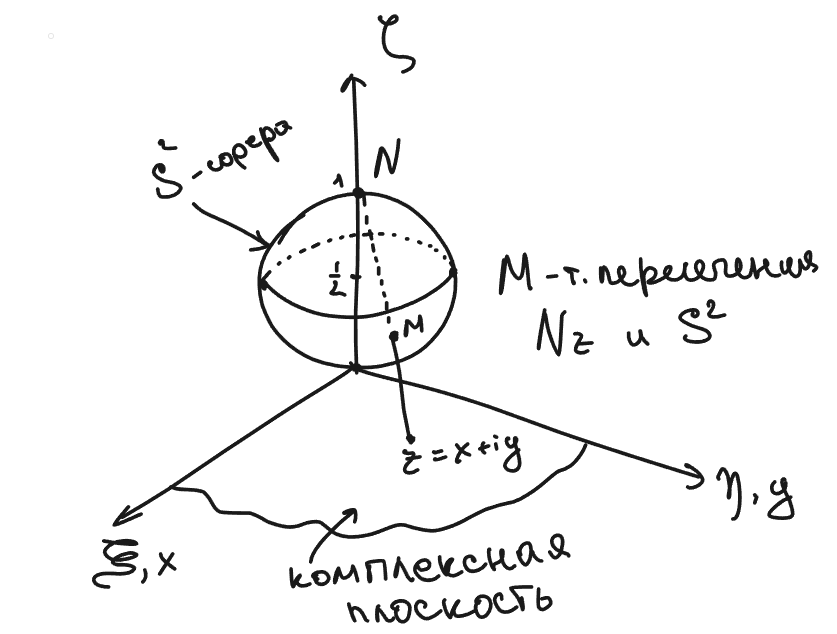
\includegraphics[scale=0.7]{answers/img/3.png}
    \label{pic04}
    \end{center}
\end{figure}
Рассмотрим сферу радиуса $\frac{1}{2}$ в этой системе координат, которая описывается уравнением 
$$
S^2: \xi^2 + \eta^2 + \left(\zeta - \frac{1}{2}\right)^2 = \left(\frac{1}{2}\right)^2
$$
а также луч, исходящий из точки $N(0,0,1)$, и пересекающий плоскость $0xy$ в точке (x,y), заданный параметрически:
$$
\begin{cases}
  \xi = 0 + tx \\
  \eta = 0 + ty \\
  \zeta = 1 + t \cdot (-1)
\end{cases}
$$

Точка пересечения луча со сферой $(\xi,\eta,\zeta)$ (подставляем в уравнение сферы уравнения луча):
\begin{gather*}
  t^2x^2 + t^2y^2 + \left(\frac{1}{2} - t\right)^2 = \left(\frac{1}{2}\right)^2 \\
  t^2(x^2 + y^2 + 1) - t = 0~~ | : t \neq 0 \\
  t = \frac{1}{1+x^2+y^2} = \frac{1}{1+|z|^2}
\end{gather*}
\begin{equation} \label{eq:forward}
\begin{cases}
  \xi = \frac{x}{1+x^2 + y^2} = \frac{x}{1+|z|^2} \\
  \eta = \frac{y}{1+x^2 + y^2} = \frac{y}{1+|z|^2} \\
  \zeta = \frac{x^2 + y^2}{1+x^2 + y^2} = \frac{|z|^2}{1+|z|^2}
\end{cases}
\end{equation}

Обратное отображение:
\begin{gather*}
\zeta = \frac{|z|^2 + 1 - 1}{1+|z|^2} \Rightarrow \frac{1}{1 + |z|^2} = 1 - \zeta \\
\Rightarrow \xi = x(1 - \zeta), \eta = y(1 - \zeta)
\Rightarrow 
\end{gather*}
\begin{equation}\label{eq:backwards}
\begin{cases}
  x = \frac{\xi}{1 - \zeta} \\
  y = \frac{\eta}{1 - \zeta}
\end{cases}
\end{equation}

Отображения (\ref{eq:forward}) и (\ref{eq:backwards}) являются однозначными отображениями между $\mathbb{C}$ и $S^2 \setminus N$, так как в преобразованиях не возникали неоднозначности.

$\overline{\mathbb{C}} = \mathbb{C} \cup \{\infty\}$. $\overline{\mathbb{C}}$ называется \textbf{расширенной комплексной плоскостью}. 

\textbf{Топология} $\overline{\mathbb{C}}$:

Открытое множество на $S^2$ -- $U \cap S^2$, где $U$ -- открытое в $\mathbb{R}^3$.

Условимся, что точке $N(0,0,1)$ соответствует точка $\infty$ поля $\overline{\mathbb{C}}$, тем самым определяется биекция между $S^2$ и $\overline{\mathbb{C}}$, точка $\infty$ называется \textbf{бесконечно удаленной точкой}.

\textbf{Окрестностью} $U$ бесконечно удаленной точки называется множество точек $z$, удовлетворяющих неравенству
$$
|z - z_0| > R, R\in \mathbb{R}
$$

Функция $f: U \rightarrow \overline{\mathbb{C}}$, $\infty\in U$, \textbf{дифференцируема в точке $\infty$}, если функция $\varphi(z) = f\left(\frac{1}{z}\right)$ дифференцируема в нуле.

Функция $f: U \rightarrow \overline{\mathbb{C}}$, $\infty\in U$, \textbf{конформна в точке $\infty$}, если функция $\varphi(z) = f\left(\frac{1}{z}\right)$ конформна в нуле.
